\section{Экспериментальное исследование}

Предложенный алгоритм был реализован на платформе .NET как часть исследовательского проекта YaccConstructor. Основным языком разработки являлся F$\#$. Был переиспользован генератор рекурсивных автоматов, реализованный ранее в рамках работы \cite{Gorokhov2017ebnf}. Также были переиспользованы структуры данных для представления структурированного в виде графа стека.

Для проверки работоспособности и оценки производительности алгоритма был проведен ряд тестов. В качестве представления шаблонов для поиска была выбрана грамматика $G_1$, задающая язык правильных скобочных последовательностей. Входные данные, в которых осуществлялся поиск, создавались следующим образом.
\begin{itemize}
	\item[1.] Из символов латинского алфавита генерировалась последовательность определенной длины, содержащая ровно пять подстрок, удовлетворяющих грамматике $G_1$.
	\item[2.] Последовательность сжималась в контекстно-свободную грамматику при помощи алгоритма Sequitur \cite{sequitur, sequitur_url}.
	\item[3.] Описание полученной грамматики транслировалось в язык YARD, используемый в проекте YaccConstructor.
\end{itemize}
В каждом тесте из серии алгоритм корректно определял наличие шаблонов, получая пять пар вершин рекурсивного автомата, построенного по входной  грамматике. 

Оценка производительности заключалась в измерении времени работы алгоритма и количества создаваемых дескрипторов (рис. \ref{time_descr}), а также объема используемой памяти, выраженного в количестве вершин и ребер GSS, построенных в процессе анализа (рис. \ref{gss}). Тестирование проводилось при различных размерах входной грамматики данных. Размером грамматики $G = (\Sigma, N, P, S)$ назовем следующую величину:
$$|G| = |N| + \sum_{p \, \in \, P} length(p)$$ 
Для тестов использовался ПК со следующими характеристиками: \linebreak MS Windows 10 x64, Intel(R) Core(TM) i7-4790 CPU @ 3.60 GHz 4 Cores, 16GB.

\begin{figure}[h]
	\centering
\begin{subfigure}[b]{0.45\textwidth}
	\centering
	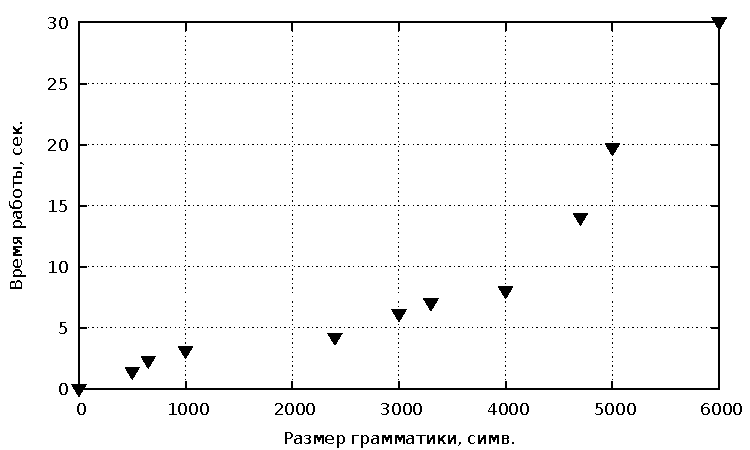
\includegraphics[width=\textwidth]{pictures/time.pdf}
	\caption{Время работы}
\end{subfigure}
~
\begin{subfigure}[b]{0.45\textwidth}
	\centering
	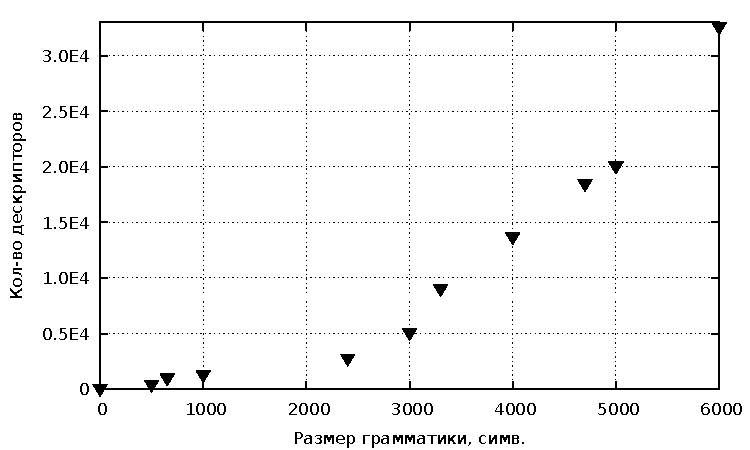
\includegraphics[width=\textwidth]{pictures/descr.pdf}
	\caption{Кол-во дескрипторов}
\end{subfigure}
\caption{Зависимость времени работы и кол-ва дескрипторов от размера входной грамматики}
\label{time_descr}
\end{figure}

\begin{figure}[h]
	\centering
	\begin{subfigure}[b]{0.45\textwidth}
		\centering
		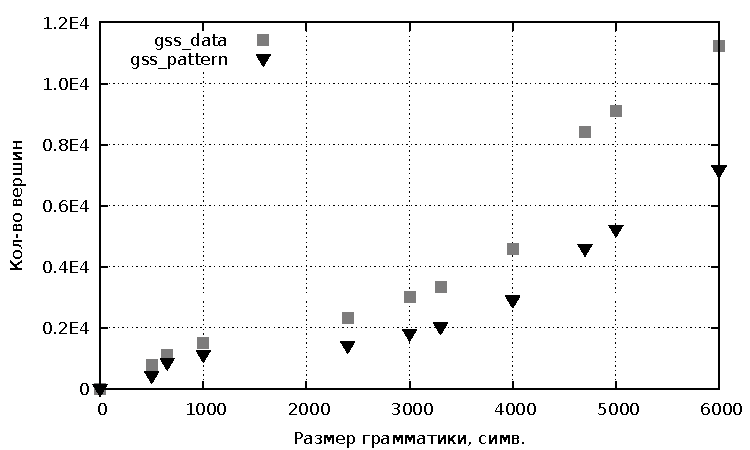
\includegraphics[width=\textwidth]{pictures/gss.pdf}
		\caption{Кол-во вершин}
	\end{subfigure}
	~
	\begin{subfigure}[b]{0.45\textwidth}
		\centering
		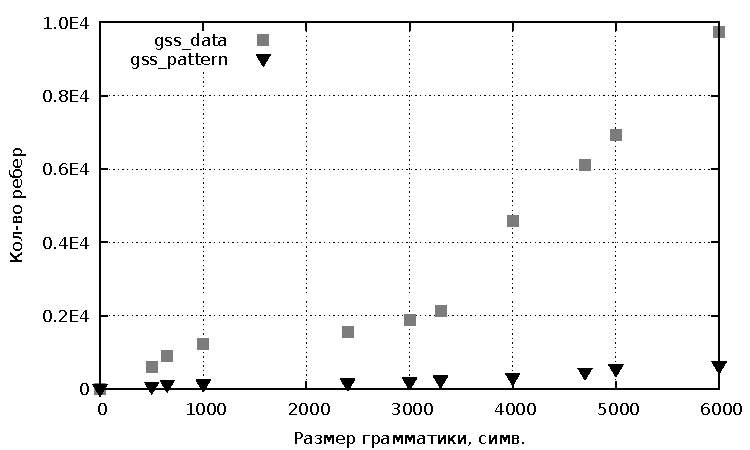
\includegraphics[width=\textwidth]{pictures/gss_edge.pdf}
		\caption{Кол-во ребер}
	\end{subfigure}
	\caption{Зависимость размера построенных GSS от размера входной грамматики. Для обозначения GSS, соответствующего грамматике $G_1$, используется метка $gss\_pattern$, входной грамматике --- $gss\_data$}
	\label{gss}
\end{figure}

Результаты тестирования показывают, что даже в случае поиска простого шаблона время работы алгоритма быстро возрастает при увеличении размеров грамматики, представляющей данные. Предположительно, производительность может быть улучшена путем технической доработки используемых структур данных и самого алгоритма. Помимо этого, влияние на работу алгоритма может оказывать не только размер входной грамматики, но и ее структура, которая зависит от используемого алгоритма сжатия.
